\documentclass[sigconf,nonacm]{acmart}
\settopmatter{printacmref=false}
\renewcommand\footnotetextcopyrightpermission[1]{}
\pagestyle{plain}
\usepackage{graphicx}
\usepackage{subcaption}
\usepackage{booktabs}

\title{Autonomous Vehicle Corner-Case Safety}
\author{Tianhang Zhu}
\affiliation{
  \institution{EE495 Autonomous Vehicles}
  \city{Evanston}
  \country{USA}
}
\author{Yiming Liu}
\affiliation{
  \institution{EE495 Autonomous Vehicles}
  \city{Evanston}
  \country{USA}
}

\begin{document}

\maketitle

\section{Rule-Priority-Conflict Scenarios}

Part B studies two unsafe scenarios in which the primary failure does not come from raw object detection alone, but from rule interpretation, lane attribution, and temporary-control arbitration under changing traffic authority \cite{mutcd2023,manuel2020,veer2022}. The common pattern is that the autonomous vehicle is exposed to stale route-level priors, locally valid temporary control, and ambiguous near-field evidence at the same time.

Unsafe behavior emerges when the stack commits too early, fails to override stale intent, or oscillates in a transition region without a stable arbitration policy \cite{shalev2017}.

\section{Unsafe Scenarios}

\subsection{B1: Signal Misread or Lane-Attribution Error at a Reversible-Lane Entrance}

B1 considers a reversible-lane entrance where overhead lane-use control signals are degraded by glare, occlusion, and viewpoint shift. The key risk is not only semantic misclassification of the signal itself, but incorrect signal-to-lane attribution. In the dominant unsafe case, an adjacent lane displays an open-looking cue while the ego lane should not inherit that authority. As a result, a permissive stack may convert a visible open cue into ego-lane passability belief even though attribution remains unresolved \cite{behrendt2017,jensen2018,hirabayashi2019,monninger2023}.

This failure has two realistic phenotypes. The first is \emph{direct premature commitment}: the system commits into the wrong lane without fully resolving attribution ambiguity. The second is \emph{critical-zone oscillation}: the system alternates between cautious hold, commit, and abort behaviors when the belief remains near threshold under contradictory evidence.

Both phenotypes are safety-relevant, because the former is a stable wrong decision while the latter produces unstable arbitration near a restricted lane entrance. Reported wrong-way AV operation in Tempe provides a real-world motivation for this failure family \cite{abc7tempe2024}.

\begin{figure}[t]
    \centering
    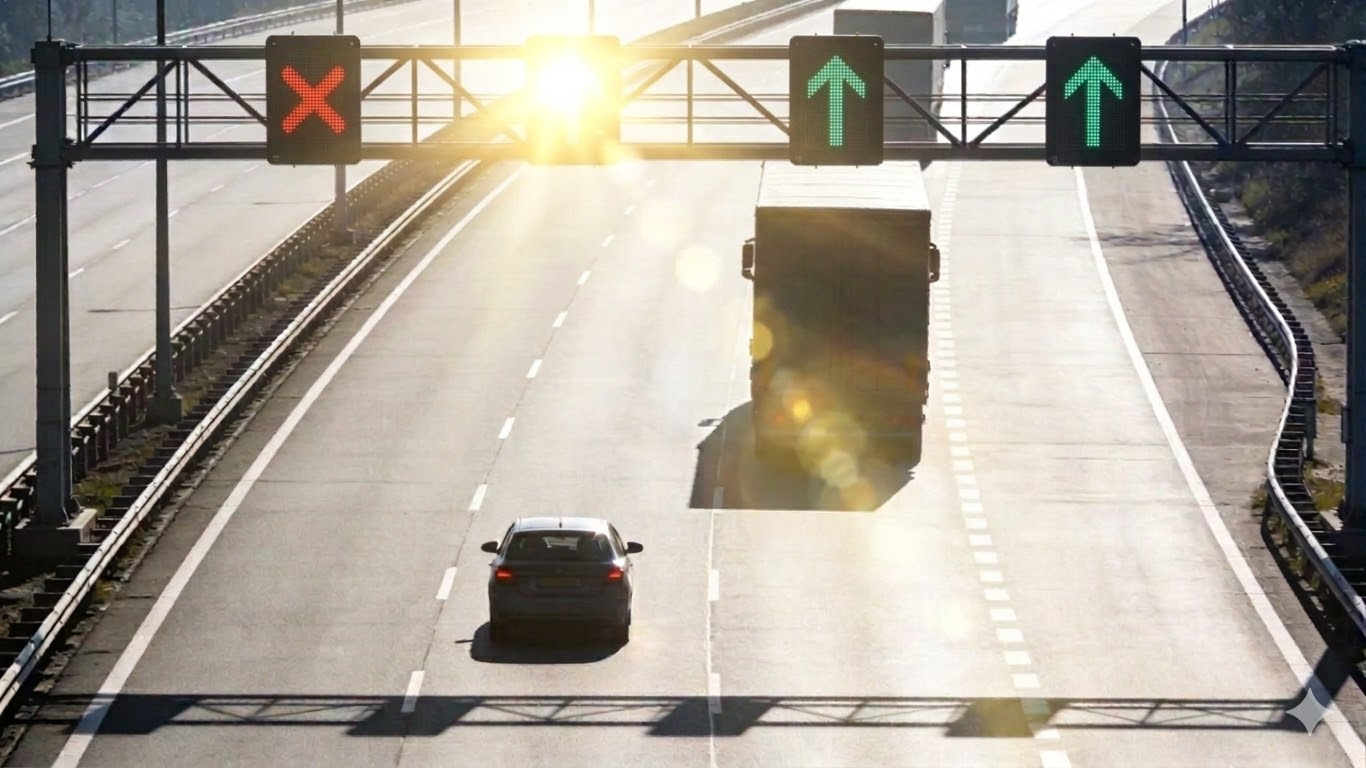
\includegraphics[width=\linewidth]{B1.png}
    \caption{Illustration of unsafe Scenario B1 at a reversible-lane entrance. Glare and limited viewing geometry degrade recognition of the overhead lane-use signal and create signal-to-lane attribution ambiguity.}
    \label{fig:b1_scene}
\end{figure}

\subsection{B2: Temporary Rerouting Conflict at a Freeway Exit During a Transition Window}

B2 considers a freeway off-ramp where the nominal route prior still suggests that staying in the rightmost lane leads to the intended exit, while near-field temporary control has already begun to close, redirect, or partially block that exit. The core risk is therefore not a missed work-zone detection in isolation, but failure to override stale exit intent during the transition window. If the original exit remains invalid but the stack continues to treat it as valid, the vehicle may commit into a closed or redirected region too late and then attempt an unstable correction \cite{mutcd2023,manuel2020}.

The desired mitigation logic for B2 is a \emph{hold-first} arbitration policy: far from the exit, the vehicle may maintain route intent or enter a preparatory state, but it should not perform a final exit commit until the local temporary control is sufficiently weak and the boundary risk remains low.

Conversely, once temporary control and boundary evidence dominate, the system should lock into a safe rerouting or merge-back mode rather than oscillating back into stale exit commitment. This is consistent with rule-hierarchy and RSS-style conservative arbitration ideas, but adapted to transition-window authority conflict \cite{mutcd2023,veer2022,shalev2017}. Real-world degraded-control behavior from Waymo vehicles during a San Francisco power outage provides a practical B2-aligned motivation \cite{ap2025waymopower}.

\begin{figure}[t]
    \centering
    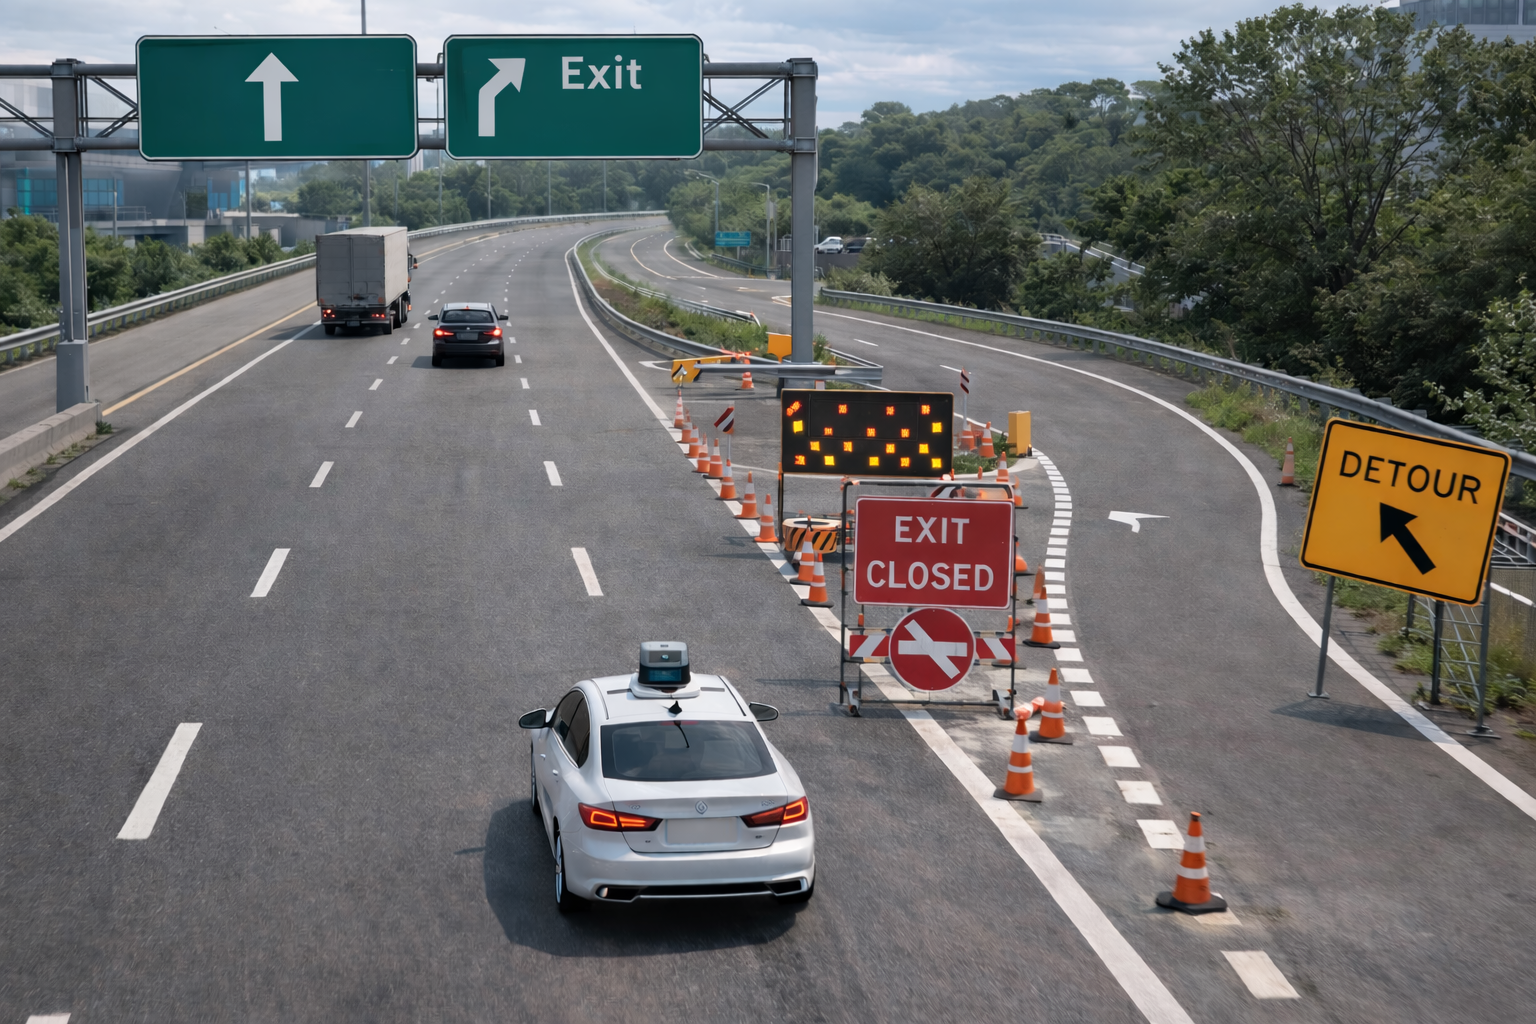
\includegraphics[width=\linewidth]{B2.png}
    \caption{Illustration of unsafe Scenario B2 at a freeway exit during a transition window. Stale exit guidance conflicts with temporary rerouting control near the ramp entry.}
    \label{fig:b2_scene}
\end{figure}

\section{Phenomenological Simulation Setup}

Part B uses a lightweight closed-loop simulator aligned with the Part A modeling philosophy. Instead of simulating full visual rendering or high-fidelity traffic scenes, the simulator directly parameterizes corner-case evidence at the fusion and planning interface. This choice preserves control over the failure mechanism and allows fair architecture comparison under identical randomized cases, while remaining compatible with the architecture-level perspective used in recent multi-sensor fusion studies \cite{huang2022survey,centerfusion2020,transfuser2021,bevfusion2022,umoe2023}.

For both B1 and B2, one shared case is sampled once and then reused across all three architecture classes: \emph{camera-only}, \emph{multi-sensor permissive}, and \emph{mitigation}. Shared latent fields generate observed cues, and the three stacks differ only in belief update, contradiction handling, and state-transition policy. This keeps the comparison focused on arbitration logic rather than different random scene realizations.

For B1, the simulator generates a shared open-looking cue, an ego-lane attribution cue, and a conflict signal that summarizes contradictory motion or geometry evidence. The dominant unsafe case is \texttt{adjacent\_open\_risk}, where the adjacent lane carries an open-looking signal while the ego lane should not be entered. The headline metric is \textbf{Wrong Commitment Rate (WCR)}, which records whether the stack ever commits into the ego lane when the oracle state is unsafe. Additional diagnostics include the decision oscillation count (DOC), travel delay, and early-commit lead.

For B2, the simulator generates a stale exit-prior cue, a temporary-control cue, a boundary-risk cue, and a contradiction signal. The key closed-exit case is \texttt{closed\_transition\_conflict}. The headline metric is \textbf{Conflict Intrusion Rate (CIR)}, which records whether the stack ever performs an unsafe exit-commit while the exit is locally closed or already in a no-return region. A complementary metric, \textbf{Late Merge-Back Severity (LMS)}, measures how late the stack abandons the invalid exit.

\section{Results}

\subsection{B1 Results}

The B1 summary is consistent with the intended Part A-style narrative: camera-only is most vulnerable, multi-sensor permissive reduces risk but does not fully eliminate it, and mitigation is the most conservative and safest stack. Across all randomized B1 runs, the average WCR is $0.81$ for camera-only, $0.05$ for multi-sensor permissive, and $0.00$ for mitigation.

The corresponding DOC values are $2.80$, $2.71$, and $2.34$, while travel delay increases from $0.201\,\mathrm{s}$ to $0.497\,\mathrm{s}$ and $0.607\,\mathrm{s}$ as the policy becomes more conservative.

The dominant \texttt{adjacent\_open\_risk} subset shows the clearest separation. In this core case, camera-only reaches a wrong commitment event rate of $1.000$, multi-sensor permissive reduces that rate to $0.062$, and mitigation drives it to $0.000$. This supports the interpretation that the main B1 failure is not simple visibility loss, but premature lane-level commitment under unresolved attribution ambiguity. Multi-sensor fusion helps, but contradiction-aware arbitration is still needed to suppress residual wrong entry.

\begin{figure}[t]
    \centering
    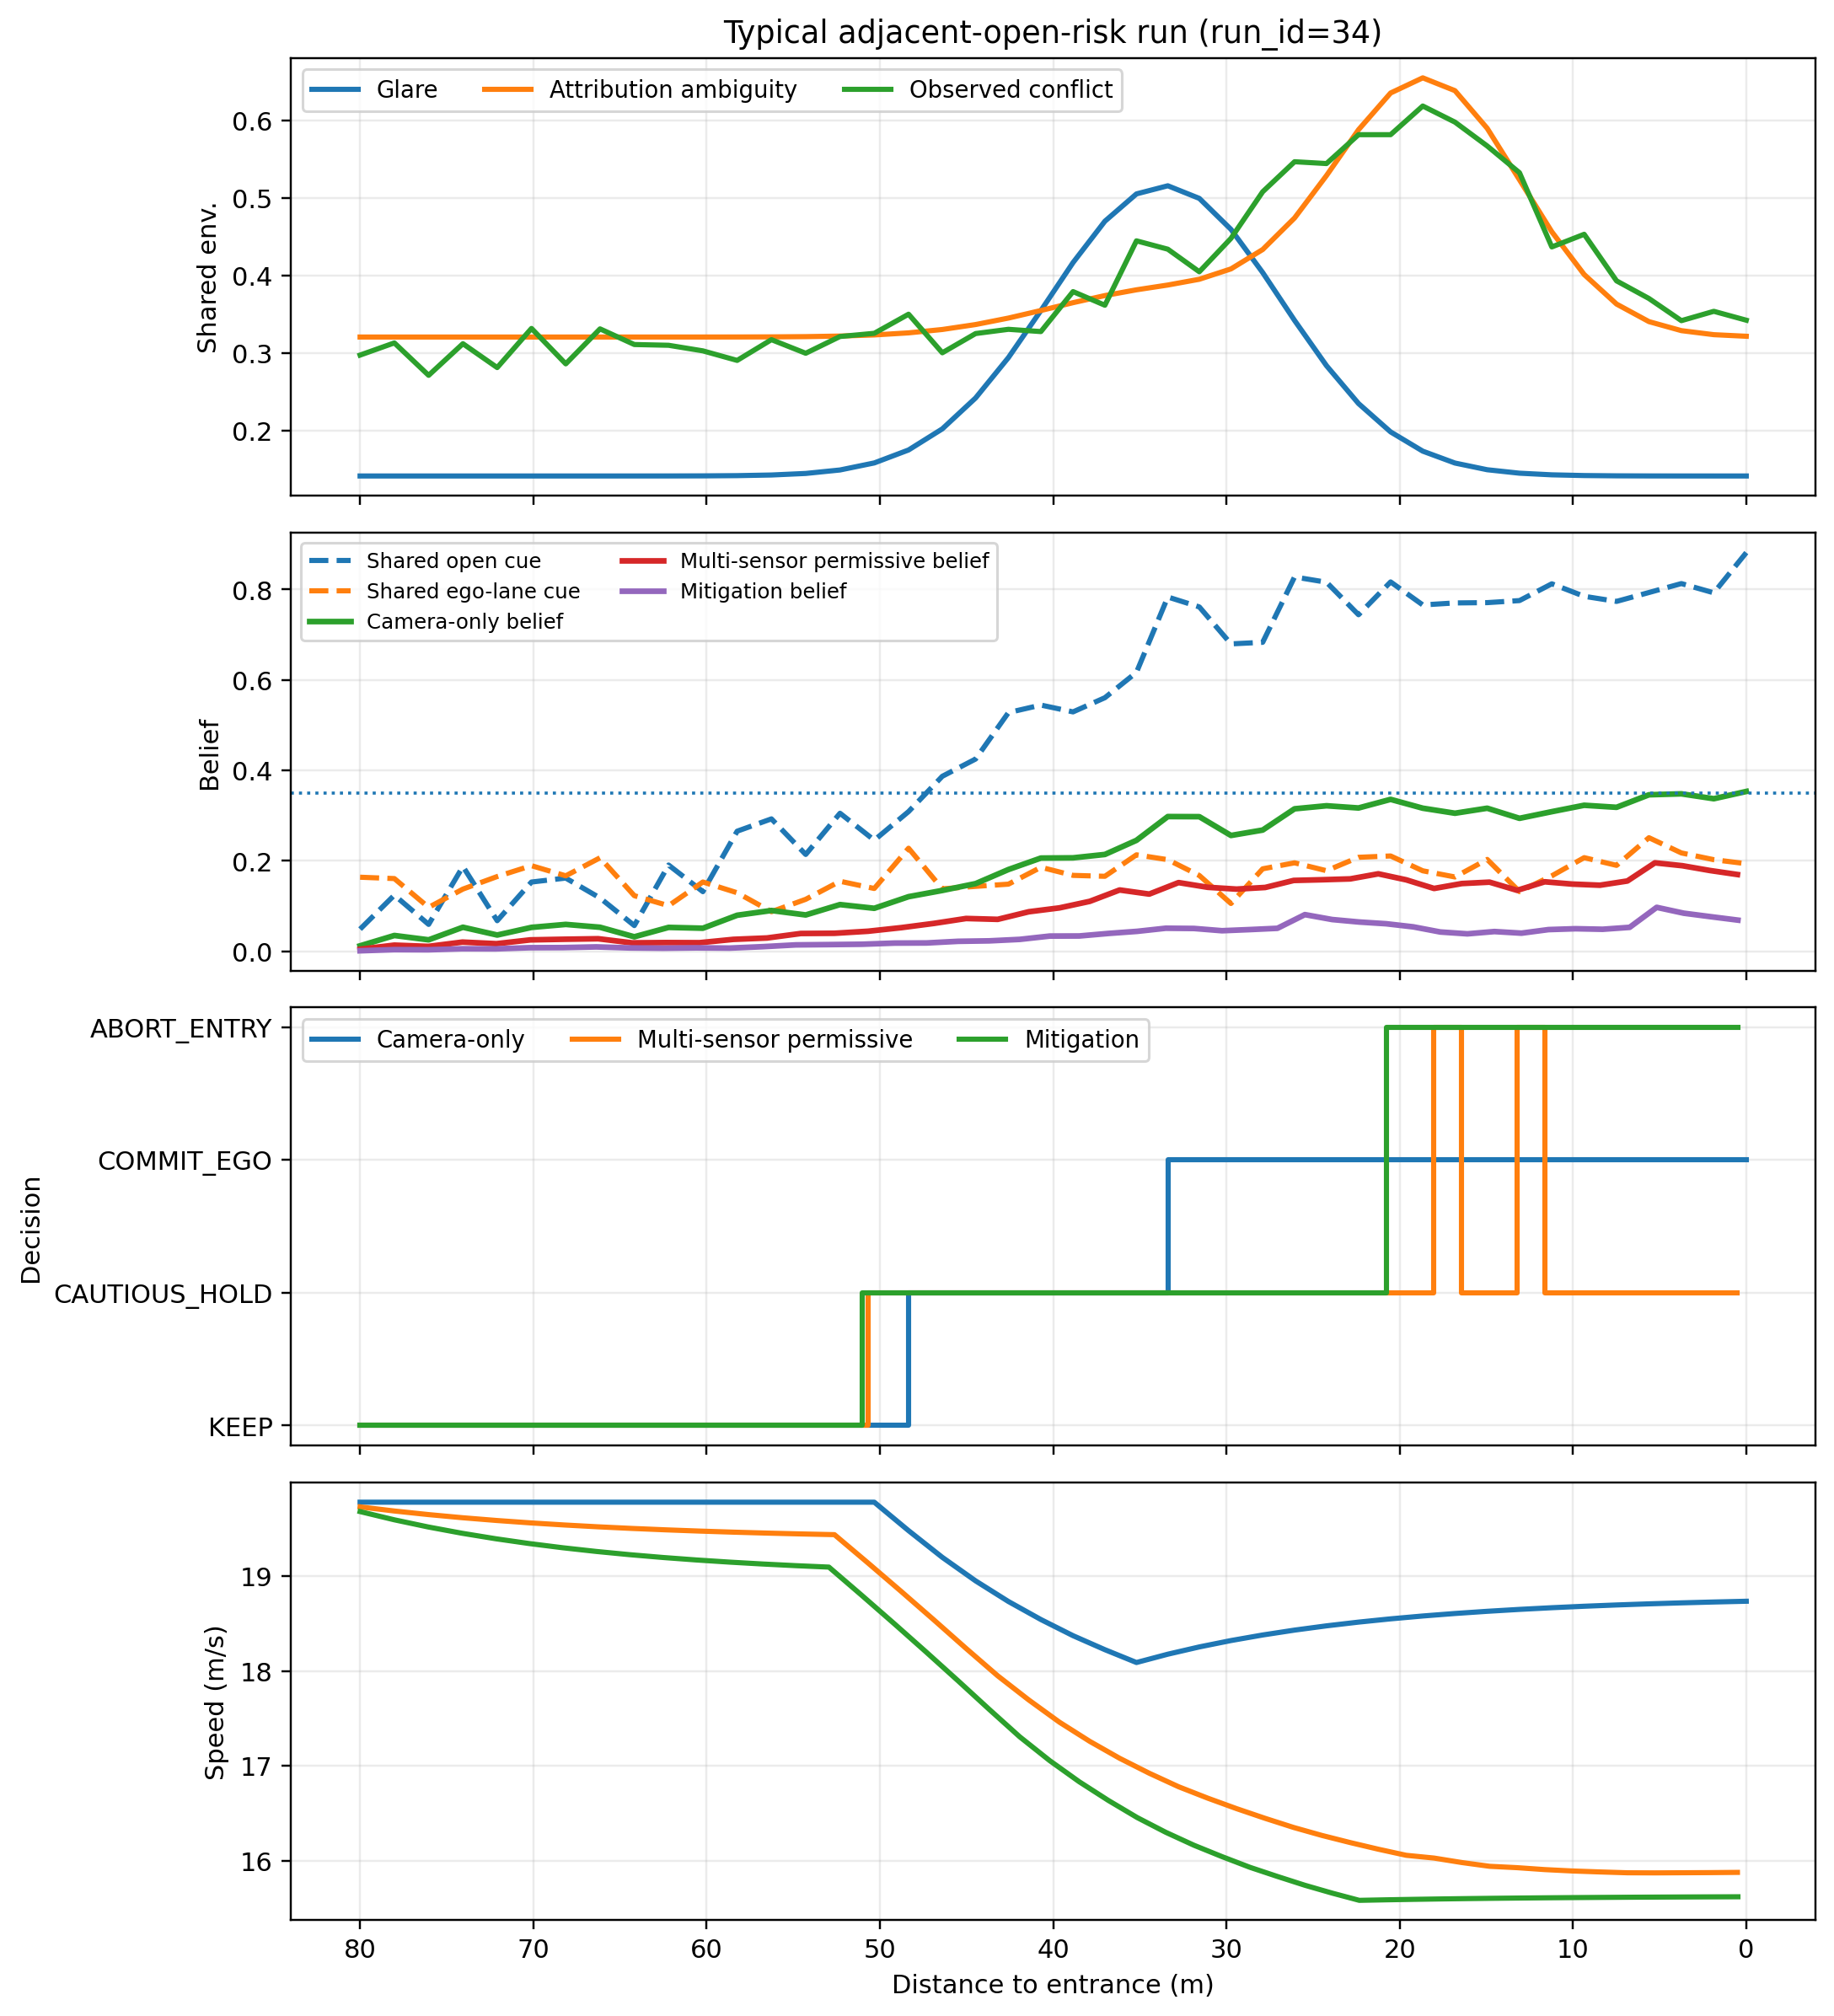
\includegraphics[width=\linewidth]{../../results_/figures/b1_aligned_partA_typical_case.png}
    \caption{Typical B1 run in the adjacent-open-risk setting. Shared cues are identical across architectures, but the arbitration policy determines whether the system commits early, oscillates, or remains conservative.}
    \label{fig:b1_typical}
\end{figure}

\begin{table}[t]
    \centering
    \caption{B1 cross-architecture summary.}
    \label{tab:b1_summary}
    \small
    \setlength{\tabcolsep}{4pt}
    \renewcommand{\arraystretch}{1.08}
    \begin{tabular}{lcccc}
        \toprule
        Architecture & WCR $\downarrow$ & DOC $\downarrow$ & $T_{\text{delay}}$ (s) $\downarrow$ & Aux. cost $\downarrow$ \\
        \midrule
        Camera-only & 0.810 & 2.800 & 0.201 & 17.043 \\
        Multi-sensor permissive & 0.050 & 2.710 & 0.497 & 1.493 \\
        Mitigation & 0.000 & 2.340 & 0.607 & 1.080 \\
        \bottomrule
    \end{tabular}
\end{table}

\subsection{B2 Results}

The B2 results are reported with emphasis on the \texttt{closed\_transition\_conflict} subset, because that is where the core unsafe mechanism is most visible. After correcting the mitigation state machine so that far-field operation remains in \texttt{KEEP\_ROUTE}, \texttt{EXIT\_PREP}, or \texttt{CAUTIOUS\_HOLD}, the ordering now matches the intended Part A-style conclusion.

In the closed-transition subset, camera-only reaches a CIR of $0.486$, multi-sensor permissive reduces this to $0.014$, and mitigation further reduces it to $0.000$.

The same subset shows a strong improvement in late correction behavior. Camera-only has an LMS of $22.429\,\mathrm{m}$, meaning that abandonment of the invalid exit is either very late or effectively missing. Multi-sensor permissive improves this to $0.398\,\mathrm{m}$, while mitigation further reduces LMS to $0.012\,\mathrm{m}$. This indicates that the mitigation is not merely less error-prone; it also performs the temporary-control override earlier and more stably.

Across the full B2 protocol, multi-sensor permissive still exhibits more arbitration churn than mitigation. In the closed-transition subset, DOC is $4.886$ for multi-sensor permissive versus $3.414$ for mitigation. This matches the intended behavioral distinction: the permissive baseline still oscillates in the transition window, whereas the mitigation uses stronger override, hysteresis, and no-return locking to stabilize the final decision.

\begin{figure}[t]
    \centering
    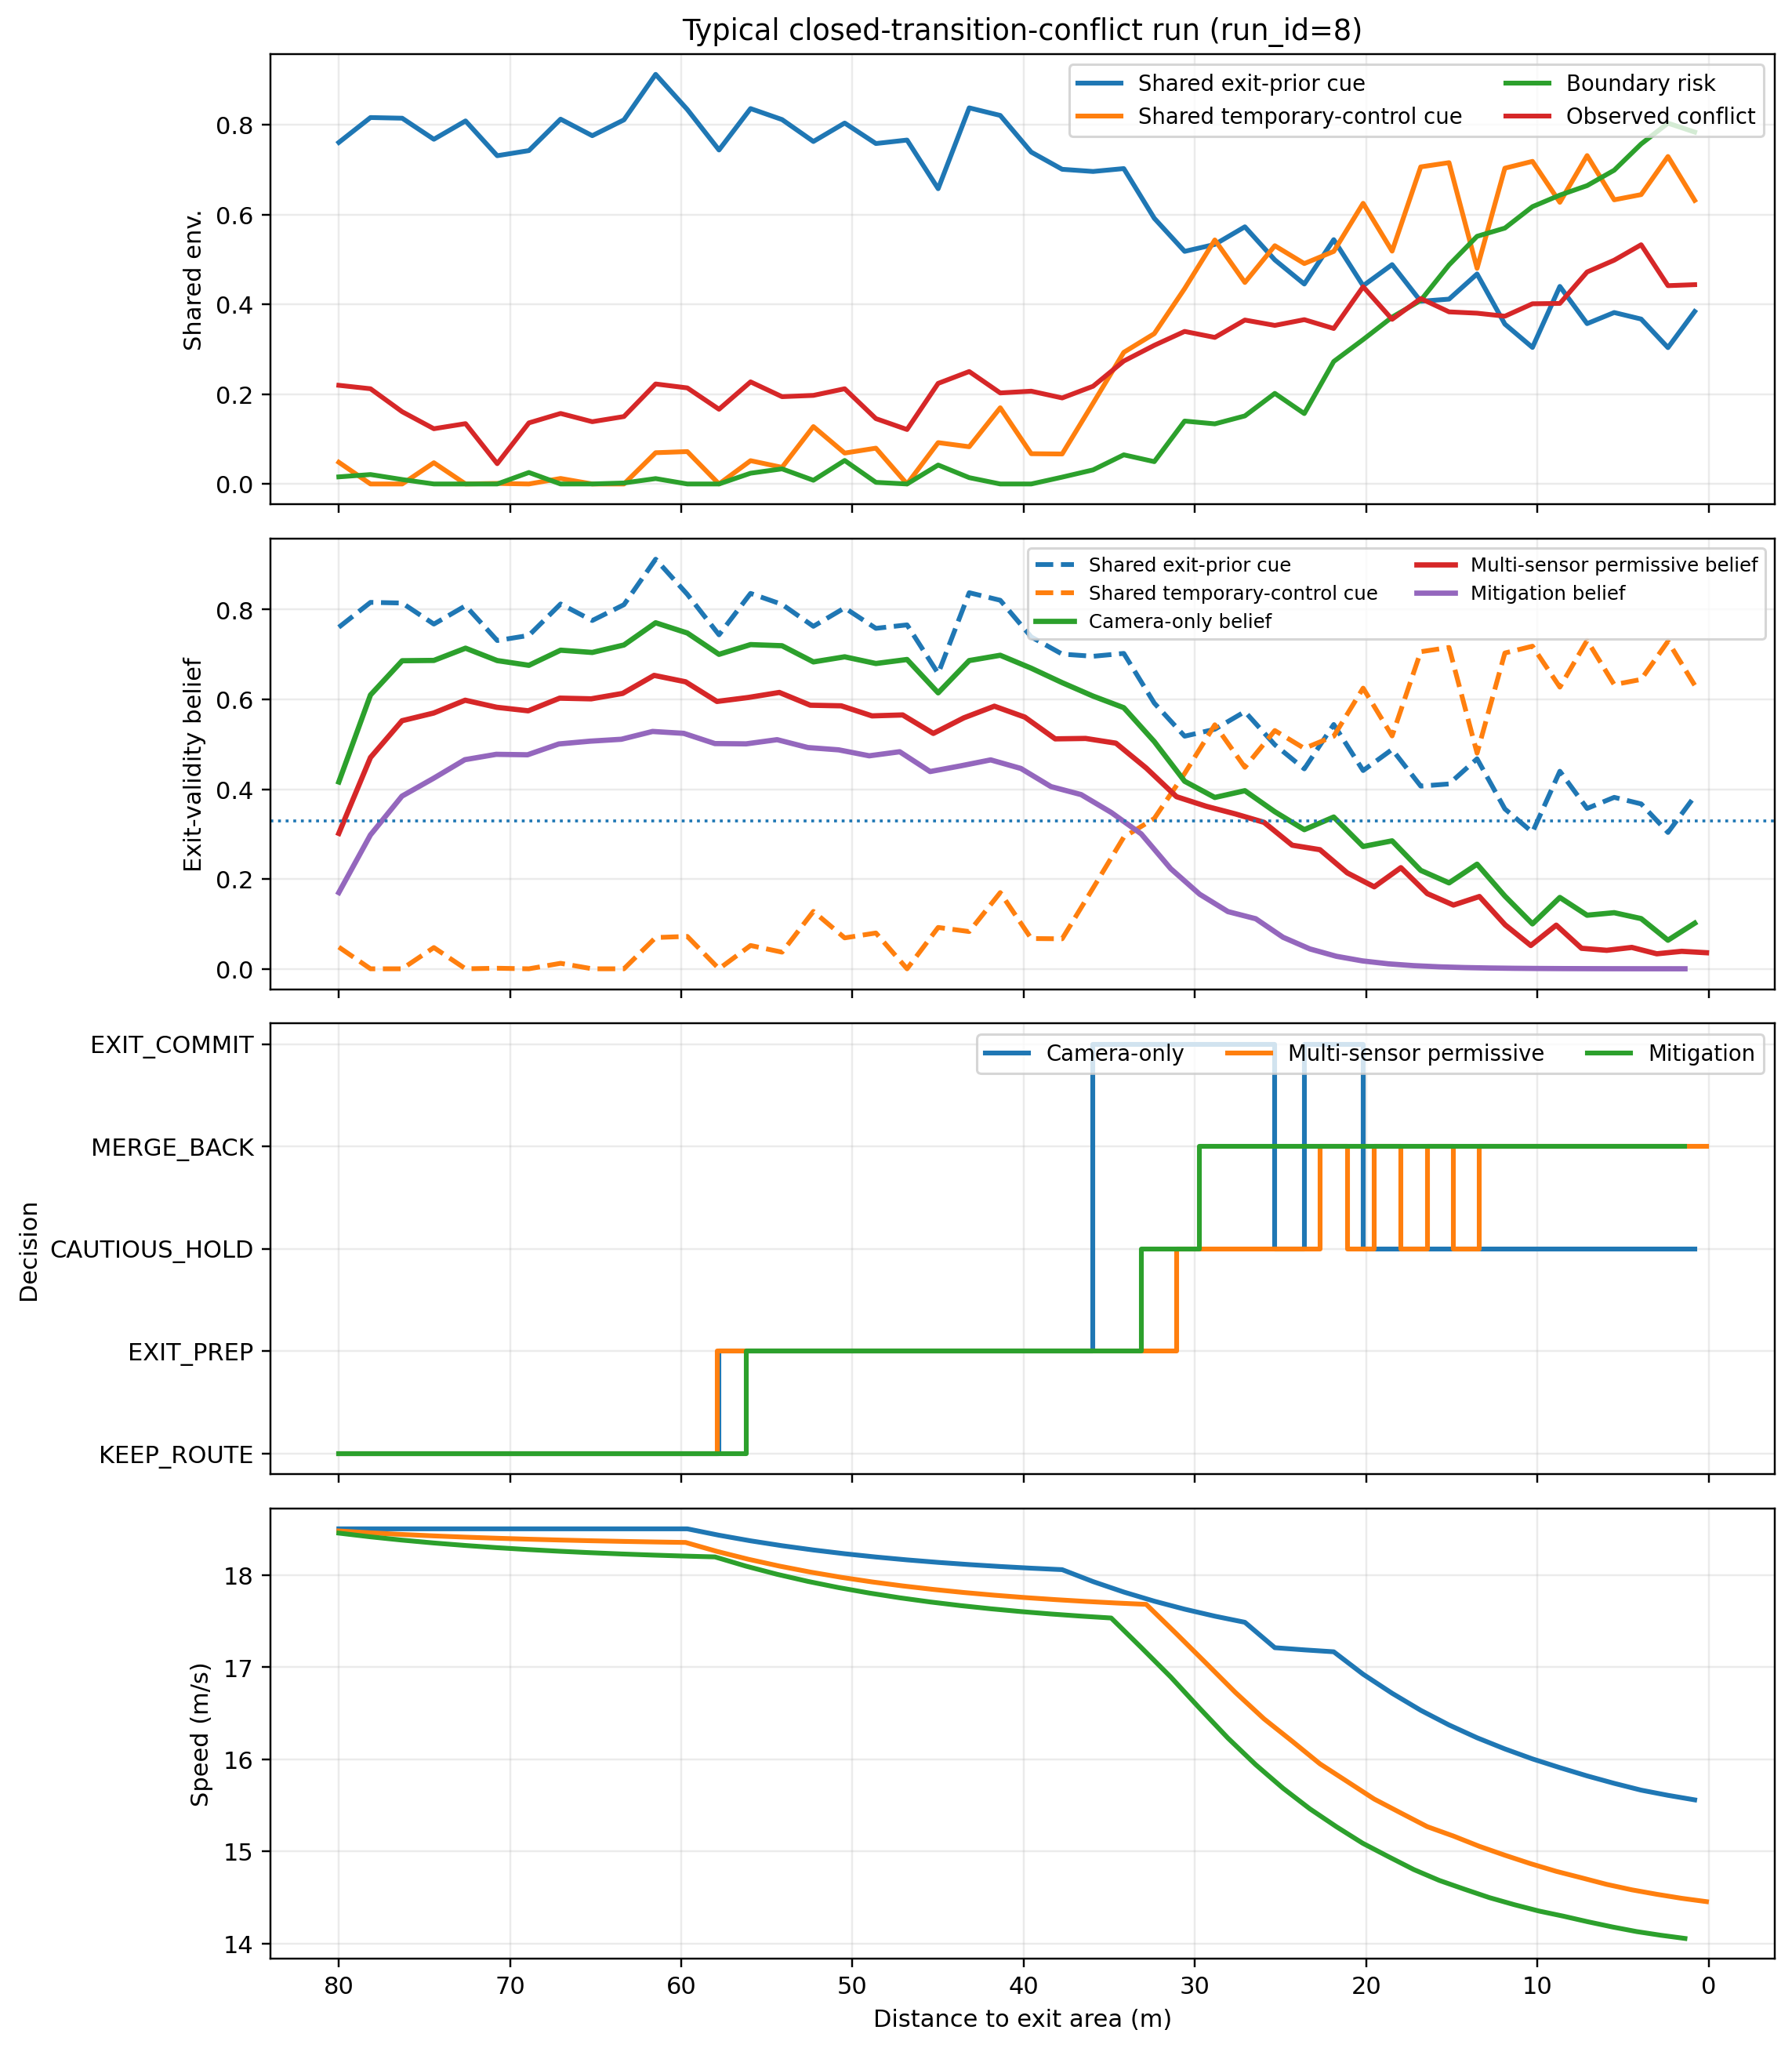
\includegraphics[width=\linewidth]{../../results_/figures/b2_aligned_partA_typical_case.png}
    \caption{Typical B2 closed-transition-conflict run. Camera-only commits too far into the stale exit prior, multi-sensor permissive shows stronger oscillation near the transition region, and mitigation switches earlier into a stable safe fallback.}
    \label{fig:b2_typical}
\end{figure}

\begin{table}[t]
    \centering
    \caption{B2 closed-transition-conflict summary.}
    \label{tab:b2_summary}
    \small
    \setlength{\tabcolsep}{4pt}
    \renewcommand{\arraystretch}{1.08}
    \begin{tabular}{lcccc}
        \toprule
        Architecture & CIR $\downarrow$ & DOC $\downarrow$ & $T_{\text{delay}}$ (s) $\downarrow$ & LMS (m) $\downarrow$ \\
        \midrule
        Camera-only & 0.486 & 3.629 & 0.279 & 22.429 \\
        Multi-sensor permissive & 0.014 & 4.886 & 0.407 & 0.398 \\
        Mitigation & 0.000 & 3.414 & 0.489 & 0.012 \\
        \bottomrule
    \end{tabular}
\end{table}

\section{Mitigation Strategies}

\subsection{Mitigation Summary and Philosophy}

The Part B mitigation philosophy follows the same logic as Part A: the main problem is not a missing detector in isolation, but premature commitment under unresolved contradiction. For rule-priority corner cases, the corresponding design shift is from \emph{semantic trust} to \emph{authority-aware arbitration}. The stack should not only estimate what a local cue means, but also whether that cue has enough spatial attribution, temporal persistence, and control authority to override route priors or previous intent \cite{veer2022,shalev2017}. In both B1 and B2, the mitigation therefore acts at the fusion-to-planning interface rather than only at the raw perception layer.

\subsubsection{B1 Mitigation: Attribution-Gated Commitment and Multi-Frame Confirmation}

For B1, the dominant risk is that an open-looking overhead cue is converted into ego-lane commitment before lane attribution is sufficiently resolved. The mitigation should therefore prevent direct conversion from ``signal looks open'' to ``ego lane is open.'' Instead, commitment should be gated by three coupled conditions:
\begin{itemize}
    \item \textit{Lane-level attribution confidence.} An open-looking signal should be associated with the ego lane only after explicit geometric assignment using lane topology, map priors, or structured traffic-light-to-lane association \cite{hirabayashi2019,monninger2023}.
    \item \textit{Temporal confirmation.} A single high-confidence frame is insufficient. The stack should require multi-frame persistence before entering a committed lane-following state.
    \item \textit{Contradiction-aware fallback.} If motion cues, occlusion, or attribution ambiguity remain high, the system should remain in cautious hold or abort-entry mode rather than promoting the signal into lane authority.
\end{itemize}

\textbf{Theoretical Prototype (2D Simulation):} In the current B1 simulator, the mitigation implements a guarded confirmation policy rather than a permissive threshold crossing. This drives WCR from $0.81$ in camera-only and $0.05$ in multi-sensor permissive to $0.00$ in mitigation, while accepting a moderate increase in travel delay.

\textbf{Real-World Extension:} In deployment, B1 mitigation should combine perception and topology:
\begin{itemize}
    \item \textit{Map-constrained signal attribution.} Overhead signals should be matched to candidate lanes using calibrated geometry and HD map structure rather than image appearance alone \cite{hirabayashi2019}.
    \item \textit{Visibility-aware uncertainty inflation.} When glare, occlusion, or viewpoint compression is high, the assignment confidence should be down-weighted even if the semantic classifier remains confident \cite{behrendt2017,jensen2018}.
    \item \textit{Safe-lane fallback.} If attribution remains unresolved near the entrance, the planner should default to the currently known-safe lane and explicitly forbid entering the reversible lane.
\end{itemize}

\subsubsection{B2 Mitigation: Hold-First Transition Arbitration with Override Locking}

For B2, the key hazard is stale exit intent surviving too far into a temporary-control transition window. The mitigation must therefore be \emph{hold-first}: far from the exit, the stack may preserve route intent or prepare for a possible exit, but it must not finalize exit commitment until local temporary-control and boundary evidence remain weak. Once temporary control becomes dominant, the mitigation should override stale route priors, reset any previous exit-confirmation state, and lock into rerouting if needed.

\textbf{Theoretical Prototype (2D Simulation):} The B2 mitigation is implemented as a transition-state controller with four main elements:
\begin{itemize}
    \item \textit{Far-field restriction.} The system does not allow final \texttt{EXIT\_COMMIT} in the far field; it remains in \texttt{KEEP\_ROUTE}, \texttt{EXIT\_PREP}, or \texttt{CAUTIOUS\_HOLD}.
    \item \textit{Near-field commit gating.} Exit commitment is allowed only near the ramp and only when temporary-control, boundary-risk, and contradiction cues all remain below conservative thresholds.
    \item \textit{Early override.} Once temporary-control or boundary-risk evidence exceeds the override condition, the mitigation clears previous exit-confirmation memory and accumulates reroute authority.
    \item \textit{No-return locking.} If override persists or the vehicle approaches the no-return region, the controller locks into \texttt{MERGE\_BACK} and forbids re-entry into stale exit commitment.
\end{itemize}

This policy reduces the closed-transition-conflict CIR from $0.486$ in camera-only and $0.014$ in multi-sensor permissive to $0.000$ in mitigation, while also reducing LMS from $22.429\,\mathrm{m}$ to $0.012\,\mathrm{m}$.

\textbf{Real-World Extension:} In higher-fidelity operation, the same idea should be expressed as authority-aware state arbitration:
\begin{itemize}
    \item \textit{Temporary-control dominance.} Cones, arrow boards, barricades, and temporary signs should be treated as local high-authority control that can override stale route semantics \cite{fhwa2008,fhwa2019}.
    \item \textit{Hysteresis and dwell-time.} Transition decisions should require short persistence windows in order to suppress planner thrashing under rapidly changing local evidence \cite{shalev2017}.
    \item \textit{Irreversibility near the gore.} Once local closure cues dominate near the no-return zone, the planner should explicitly forbid a return to exit-commit behavior.
\end{itemize}

\section{Discussion and Conclusion}

The main conclusion of Part B is that rule-priority corner cases are best understood as arbitration failures under conflicting authority, not as isolated perception misses. In B1, the key hazard is premature lane commitment under ambiguous signal attribution. In B2, the key hazard is failure to override stale route intent during a temporary-control transition window. In both cases, the camera-only stack is the most failure-prone, multi-sensor permissive fusion improves average behavior but still retains residual instability, and the mitigation performs best when it explicitly encodes cautious hold, dwell-time confirmation, contradiction-aware override, and no-return locking \cite{hirabayashi2019,monninger2023,veer2022,shalev2017}.

\begin{thebibliography}{18}

\bibitem{abc7tempe2024}
ABC7 Chicago.
\newblock 2024.
\newblock \textit{Self-Driving Waymo Car Goes Wrong Way into Oncoming Traffic in Arizona}.
\newblock \url{https://abc7chicago.com/post/wrong-waymo-driverless-car-goes-oncoming-traffic-tempe-arizona/15238556/}.

\bibitem{ap2025waymopower}
Associated Press.
\newblock 2025.
\newblock \textit{Waymos Blocked Roads and Caused Chaos During San Francisco Power Outage}.
\newblock \url{https://apnews.com/article/81e6a00aa2be6b804fe0bdfbcf07401f}.

\bibitem{huang2022survey}
K. Huang, C. Fu, and X. Wang.
\newblock 2022.
\newblock Multi-sensor Fusion for Auto Driving Perception: A Survey.
\newblock \textit{arXiv preprint arXiv:2202.02703}.

\bibitem{mutcd2023}
Federal Highway Administration.
\newblock 2023.
\newblock \textit{Manual on Uniform Traffic Control Devices (MUTCD), 11th Edition}.

\bibitem{manuel2020}
A. Manuel, A. de Barros, and R. Tay.
\newblock 2020.
\newblock Traffic safety meta-analysis of reversible lanes.
\newblock \textit{Accident Analysis \& Prevention} 148 (2020), 105751.

\bibitem{behrendt2017}
K. Behrendt and L. Novak.
\newblock 2017.
\newblock A deep learning approach to traffic lights: Detection, tracking, and classification.
\newblock In \textit{Proc. IEEE ICRA}.

\bibitem{jensen2018}
M. Jensen et al.
\newblock 2018.
\newblock The DriveU Traffic Light Dataset: Introduction and Comparison with Existing Datasets.
\newblock In \textit{Proc. IEEE ICRA}.

\bibitem{hirabayashi2019}
M. Hirabayashi et al.
\newblock 2019.
\newblock Traffic light recognition using high-definition map features.
\newblock \textit{Robotics and Autonomous Systems} 111 (2019), 62--72.

\bibitem{monninger2023}
M. Monninger et al.
\newblock 2023.
\newblock Traffic-Light-to-Lane Assignment in Structured Urban Environments.
\newblock \textit{arXiv preprint arXiv:2309.12087}.

\bibitem{veer2022}
S. Veer et al.
\newblock 2022.
\newblock Receding Horizon Planning with Rule Hierarchies for Autonomous Vehicles.
\newblock \textit{arXiv preprint arXiv:2212.03323}.

\bibitem{shalev2017}
S. Shalev-Shwartz, S. Shammah, and A. Shashua.
\newblock 2017.
\newblock On a Formal Model of Safe and Scalable Self-driving Cars.
\newblock \textit{arXiv preprint arXiv:1708.06374}.

\bibitem{centerfusion2020}
R. Nabati and H. Qi.
\newblock 2020.
\newblock CenterFusion: Center-based Radar and Camera Fusion for 3D Object Detection.
\newblock \textit{arXiv preprint arXiv:2011.04841}.

\bibitem{transfuser2021}
A. Prakash, K. Chitta, and A. Geiger.
\newblock 2021.
\newblock Multi-sensor Fusion Transformer for End-to-End Autonomous Driving.
\newblock \textit{arXiv preprint arXiv:2104.09224}.

\bibitem{bevfusion2022}
Z. Liu et al.
\newblock 2022.
\newblock BEVFusion: Multi-Task Multi-Sensor Fusion with Unified Bird's-Eye View Representation.
\newblock \textit{arXiv preprint arXiv:2205.13542}.

\bibitem{umoe2023}
Y. Lou, Q. Song, Q. Xu, R. Tan, and J. Wang.
\newblock 2023.
\newblock Uncertainty-Encoded Multi-Modal Fusion for Robust Object Detection in Autonomous Driving.
\newblock \textit{arXiv preprint arXiv:2307.16121}.

\end{thebibliography}

\end{document}
